\documentclass[../main.tex]{subfiles}

\begin{document}
\part{ND280 upgrade}
\label{pt:up}

\chapter{Motivation}
As mentioned in the \autoref{part:T2K:general}, the initial goal of the T2K experiment was to measure the $\theta{13}$ mixing angle. The non-zero value of this angle would open a road towards the CP--violation in the neutrino oscillations. After the successful discovery of the $\theta_{13}$ T2K entered a phase of the precise measurement of the neutrino oscillation parameters. The T2K provides the most precise estimations for the $\theta_{23}$ and also very accurate measurements of the $\Delta m_{23}$ and $\theta_{13}$. The big progress was obtained in the search for the CP--violation with determination of the 3$\sigma$ confidence level on the possible values of the $\delta_{CP}$~\cite{Abe2020n}. The $\delta_{CP}$ measurement became a main goal of the experiment.

Next generation experiments like DUNE~\cite{Acciarri2016} and Hyper-Kamiokande~\cite{Proto-Collaboration2018} will be able to achieve 3$\sigma$ sensitivity to the CP--violation across the wide range of the $\delta_{CP}$ values but on the time scale 2026 and beyond. The T2K experiment has possibility to probe this effect with less sensitivity but much earlier. The sensitivity of the T2K experiment with the total statistics of $20\times10^{21}$ POT is shown in \autoref{fig:up:sens}.

\begin{figure}[!ht]
  \centering
  \begin{minipage}{0.49\linewidth}
    \centering
    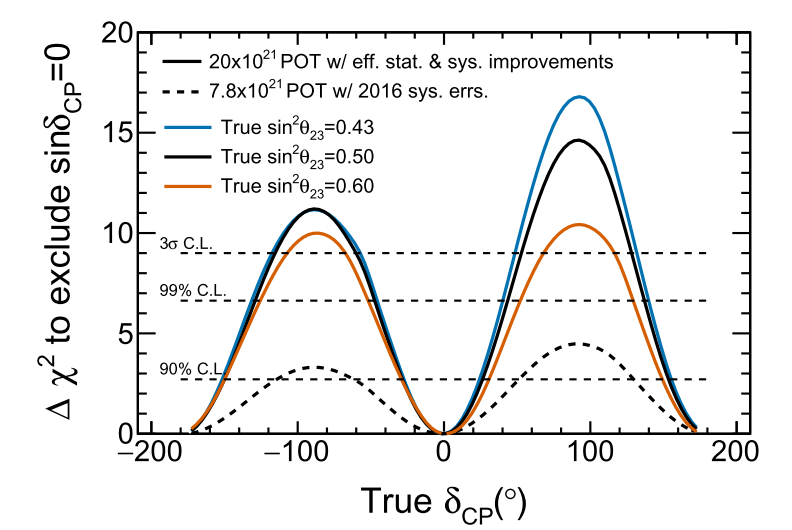
\includegraphics[width = \linewidth]{t2kII_dcp} \\ (a)
  \end{minipage}
  \begin{minipage}{0.49\linewidth}
    \centering
    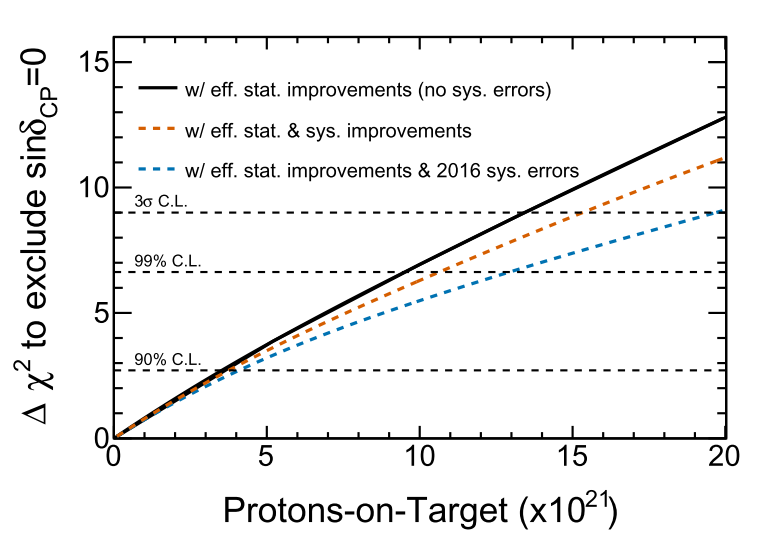
\includegraphics[width = \linewidth]{t2k_cp} \\ (b)
  \end{minipage}
    \caption{An expected sensitivity of the T2K experiment to the CP--violation in the neutrino oscillations. The known mass order is assumed. Three systematic uncertainties estimations are used: (blue) 2016 value, (orange) with expected improvements and (black) only stat. uncertainties. (a) shows the sensitivity over the $\delta_{CP}$ value and (b) shows the sensitivity evolution over the collected statistics for $\delta_{CP}=-\pi/2$.}
    \label{fig:up:sens}
\end{figure}


More statistics is necessary to determine the neutrino/anti-neutrino asymmetry more precisely and do justify if the effect takes place. For this the extended run of the T2K experiment was proposed~\cite{Abe2016e}. The next


The further improvement of the precision is limited by the systematic uncertainty of the experiment. The statistical uncertainty of the T2K experiment is still bigger than the systematic one, but the latter affect the result accuracy more and more severe. The near detector of the T2K plays a critical rope in the uncertainty reduction. With the data from ND280 the

\section{T2K run plan}
\section{Beamline upgrade}
\section{Limits of the near detector}
\chapter{Detector overview}
\chapter{Simulations}

\chapter{TPC}
\section{Concept}
\subsection{Resistive MicroMegas technology}
\section{Beamtest}
\subsection{Cosmic test}
\subsection{CERN beamtest}
\subsection{DESY beamtest}


\chapter{Super FGD}
\section{Concept}
\subsection{Assembly}
\section{Simulations}
\subsection{Expected light yield}
\subsection{Michell electron tagging}
\subsection{Pileups}
\section{Beamtest}
\subsection{First CERN beamtest}
\subsection{Second CERN beamtest}

\chapter{Neutron tagging in SuperFGD}
\section{Motivation}
\section{Geant4 simulation}
\section{Efficiency and energy resolution}
\section{Background estimatiuonsn}
\section{Prospects for physics}
\end{document}